%%\documentclass{article}
\documentclass[12pt,twoside,a4paper]{scrbook}

\usepackage{geometry}
%\usepackage{amsmath, amssymb, amsthm}
\usepackage{graphicx}
\usepackage{color}
%\usepackage{ifthen}
%\usepackage{wrapfig}
%\usepackage{framed}
\usepackage{framed}
%\usepackage{enumitem}
\usepackage{listings} 
\usepackage{hyperref}
%\usepackage[numbers,sort&compress]{natbib} 


\geometry{left=3.5cm,textwidth=15cm,top=3cm,textheight=23cm}


\newenvironment{history}
{
 \begin{framed}
  \begin{minipage}{0.9\textwidth}
   { \footnotesize
    Historic remark:
   }
}
{
  \end{minipage}
 \end{framed}  
}


\lstdefinelanguage{cCCode}[]{C}{
  basicstyle=\small,
  stringstyle=\color{red},
  keywordstyle=\color{blue},
  commentstyle=\color{grey}\slshape,
  morekeywords={linestyle,linetype,linewidth,linecolor,pointtype,nohidden3d,hidden3d,palette,lt,lw,lc,pt,ps,fd,fill,fs,ls},
  framexleftmargin=1mm, framextopmargin=1mm, frame=shadowbox,
  rulesepcolor=\color{grey}
}
    
    
\lstnewenvironment{code}[1][]{
\lstset{
 language=cCCode,#1
}}{}
    
    

%
% Miriam hat 16 Seiten und dann pro Paper eine Seite Vorwort
% Michael hat 30 Seiten inkl einer Section pro Paper
%
%

%\newenvironment{history}
{
 \begin{framed}
  \begin{minipage}{0.9\textwidth}
   { \footnotesize
    Historic remark:
   }
}
{
  \end{minipage}
 \end{framed}  
}


\lstdefinelanguage{cCCode}[]{C}{
  basicstyle=\small,
  stringstyle=\color{red},
  keywordstyle=\color{blue},
  commentstyle=\color{grey}\slshape,
  morekeywords={linestyle,linetype,linewidth,linecolor,pointtype,nohidden3d,hidden3d,palette,lt,lw,lc,pt,ps,fd,fill,fs,ls},
  framexleftmargin=1mm, framextopmargin=1mm, frame=shadowbox,
  rulesepcolor=\color{grey}
}
    
    
\lstnewenvironment{code}[1][]{
\lstset{
 language=cCCode,#1
}}{}
    
    

\begin{document}

 
\begin{titlepage}

{ \large
  \begin{center}

  TECHNISCHE UNIVERSIT\"AT M\"UNCHEN \\
%  Technische Universit\"at M\"unchen\\
  \vspace{.3cm} 
  Department of Informatics \\
  Scientific Computing

  \vspace{4cm}
   Habilitationsverfahren Dr.~rer.~nat.~Tobias Weinzierl
  
  \vspace{1.5cm}

{\Huge
Cumulative Habilitation
}
\\
\vspace{1cm}
and 
\\
\vspace{0.6cm}
{\Huge
Progress Report\\
}

%   Dr.~rer.~nat.~Tobias Weinzierl
  \vspace{1.5cm}

%  \today
  \end{center}
}


\end{titlepage}


 \thispagestyle{empty}
 \newpage
 \cleardoublepage 

 \pagestyle{plain}
 \pagenumbering{roman}
 \chapter{Preamble}


\Peano\ is an open source framework for solvers on dynamically adaptive
Cartesian meshes.
Its core is built with C++, but many tools around it are written in Python.
\Peano\  is based upon the fact that spacetrees, a generalisation of the classical octree concept, yield a cascade of adaptive Cartesian grids. Consequently, any spacetree traversal is equivalent to an element-wise traversal of the hierarchy of the adaptive Cartesian grids. The software \Peano\  realises such a grid traversal and storage algorithm, and it provides hook-in points for applications performing per-element, per-vertex, and so forth operations on the grid. It also provides interfaces for dynamic load balancing, sophisticated geometry representations, and other features. Some properties are enlisted below.

Peano is currently available in its fourth generation. 
The development of the original set of Peano codes started around 2002.
2005-2009, we merged these codes into one Peano kernel (2nd generation). 
In 2009, I started a complete reimplementation of the kernel with special
emphasis on reusability, application-independent design and the support for rapid prototyping. 
This third generation of the code ended around 2019 when we released the
ExaHyPE code---a hyperbolic equation system solver engine which uses Peano's
AMR meshes.
The current guidebook discusses \Peano\ , which reuses ideas and lessons learned
from Peano~3 as well as lots of code buildling blocks, but can be seen as a
major rewrite starting from scratch.



\Peano\ has been the code base for multiple projects over the past years.
The most prominent one is likely ExaHyPE.
The first generation of ExaHyPE has been a stand-alone projects using Peano
as one required library or framework out of many.
The second generation, \ExaHyPE, is merged into \Peano as spin-off.
This document therefore covers \ExaHyPE, too.




\section*{Dependencies and prerequisites}

\Peano's core is plain C++17 code. 
We however use a whole set of tools around it:

\begin{itemize}
  \item GNU autotools (automake) to set up the system (required).
  \item C++17-compatible C++ compiler (required).
  \item Python3 (optional; not required if you work only with the C++
  baseline).
  \item MPI2 (optional). MPI's multithreaded support is required.
  \item Intel's Threading Building Blocks or OpenMP 5. We also can work with C++
  threads, but found their performance suboptimal.
  \item The Visualization Toolkit (VTK) if you want to use the built-in
  visualisation facilities (optional).
  \item Doxygen if you want to create HTML pages of PDFs of the in-code
  documentation.
\end{itemize}

\begin{remark}
I test and maintain \Peano\  for Linux only.
If you prefer Windows or MacOS, it should work as long as you provide the
mandatory tools from above, but I won't be able to help.
\end{remark}


\begin{center}
 \begin{tabular}{|l|l|p{8cm}|}
  \hline
   Software & Version & Remarks \\
  \hline
   GNU g++ & 7.5 or older & Works with \Peano\ core but not with some extensions
   such as \ExaHyPE. \\
   GNU g++ & 9.3.1 & Current development version. Works. \\
  \hline
   Intel icpc & 19.1 & Works with \Peano\ and all
   extensions such as \ExaHyPE. Tests with Intel Fortran have been successful,
   too. \\
  \hline
   VTK & 7--9 & Supported by \Peano. Default is 8, i.e.~if you need other
   version, you have to inform configure (see Chapter \ref{chapter:postprocessing}). \\
   \hline
   Python & 3 & Development version. Python 2 is not supported by frontend. \\
   \hline
 \end{tabular}
\end{center}

\section*{Who should read this document}

This cookbook is written similar to a tutorial in a hands-on style.
Therefore, it also contains lots of source code snippets.
If you read through a chapter, you should immediately be able to re-program the
presented details in your code and use the ideas.

Therefore, this cookbook is written for people that have a decent programming
background as well as scientific computing knowledge.
% Some background in the particular application area's algorithms for some
% chapters also is required. 
It is a cookbook that shall help readers to translate their scientific vision
into a working code quickly.


\section*{How the text is organised}

% This book covers a variety of problems I have tackled with Peano when I wrote
% scientific papers.
% There is no overall read thread through the document.
% I recommend to start reading some chapters and then jump into chapters
% that are of particular interest.
% Whenever something comes to my mind that should be added, I will add it.
If you feel something is urgently missing and deserves a chapter or things
remain unclear, please write me an email and I'll see whether I can provide some
additional text or extend the cookbook.


{
  \flushright
  \today 
  \\ 
  Tobias Weinzierl 
  \\
}

 

 \cleardoublepage 
 
 \tableofcontents

 \newpage

 \cleardoublepage 

 \pagestyle{plain}
 \pagenumbering{arabic}



 \chapter{Quickstart}
\label{chapter:quickstart}


\chapterDescription
  {
    Should take you around 15 minutes to get the
    code up and running. Then another 15 minutes to have the first static
    adaptive Cartesian grid.
  }
  {
    No previous knowledge, but some experience with the Linux
    command line and Paraview is advantageous.
  }



\section{Download and install}

To start work with Peano, you need at least two things.

\begin{enumerate}
  \item The Peano source code. Today, the source code consists of two important
  directories. The \texttt{peano} directory holds the actual Peano code. An
  additional \texttt{tarch} directory holds Peano's technical architecture.
  \item The Peano Development Toolkit (PDT). The PDT is a small Java archive. It
  takes away the cumbersome work to write lots of glue code, i.e.~empty
  interface implementations, default routines, \ldots, so we use it quite
  frequently.
\end{enumerate}

\noindent
For advanced features, you might want to use some {\bf toolboxes}.
A toolbox in Peano is a small collection of files that you store in a directory
and adopt all pathes accordingly.
From a user's point of view, when we use the term toolbox we actually mean this
directory with all its content.



\begin{remark}
Originally, we hoped that Peano's technical architecture (\texttt{tarch}) might
become of value for several projects, i.e.~projects appreciate that they do not
have to re-develop things such as logging, writing of output files, writing
support for OpenMP and TBB, and so forth.
To the best of our knowledge, the tarch however is not really used by someone
else, so we cannot really claim that it is independent of Peano.
Nevertheless, we try to keep it separate and not to add anyting AMR or
grid-specific to the tarch.
\end{remark}

There are two ways to get hold of Peano's sources and tools. You either {\em
download the archives from the website} or you {\em access the repository
directly}.
Both variants are fine.
We recommend to access the respository directly.


\subsection{Download the archives from the website}

If you don't want to download Peano's whole archive, change to Peano's webpage
\url{http://www.peano-framework.org} and grab the files
\begin{itemize}
  \item \texttt{peano.tar.gz} and
  \item \texttt{pdt.jar}
\end{itemize}
from there. If you do so, please skip the first two lines from the script
before. Otherwise, load down the important files with \texttt{wget}. 
Independent of which variant you follow, please unpack the \texttt{peano.tar.gz}
archive. 
It holds all required C++ sources.

\begin{code}
> wget http://sourceforge.net/projects/peano/files/peano.tar.gz
> wget http://sourceforge.net/projects/peano/files/pdt.jar
> tar -xzvf peano.tar.gz
\end{code}


\noindent
There's a couple of helper files that we use IN the
cookbook. 
They are not necessarily required for each Peano project, but for our examples
here they are very useful.
So, please create an additional directory \texttt{usrtemplates} and grap
these files

\begin{code}
> mkdir usrtemplates
> cd usrtemplates
> wget http://sourceforge.net/projects/peano/files/ \
  usrtemplates/VTKMultilevelGridVisualiserImplementation.template 
> wget http://sourceforge.net/projects/peano/files/ \
  usrtemplates/VTKMultilevelGridVisualiserHeader.template 
> wget http://sourceforge.net/projects/peano/files/ \
  usrtemplates/VTKGridVisualiserImplementation.template 
> wget http://sourceforge.net/projects/peano/files/ \
  usrtemplates/VTKGridVisualiserHeader.template 
> wget http://sourceforge.net/projects/peano/files/ \
  usrtemplates/VTK2dTreeVisualiserImplementation.template 
> wget http://sourceforge.net/projects/peano/files/ \
  usrtemplates/VTK2dTreeVisualiserHeader.template 
\end{code}

\subsection{Access the repository directly}

Instead of a manual download, you might also decide to download a copy of the
whole Peano repository. 
This also has the advantage that you can do a simple \texttt{svn update} anytime
later throughout your development to immediately obtain all kernel
modifications.


\begin{code}
> svn checkout http://svn.code.sf.net/p/peano/code/trunk peano
\end{code}

\noindent
Your directory structure will be slightly different than in the example above,
but this way you can be sure you grabbed everything that has been released for
Peano through the webpage ever.

The archive \texttt{pdt.jar} will be contained in \texttt{pdt}, while the two
source folders will be held by \texttt{src}.
The directory \texttt{usrtemplates} is contained in \texttt{pdt}.


\subsection{Prepare your own project}


From hereon, we recommend that you do not make any changes within Peano
repositories but use your own directory \texttt{peano-projects} for your own
projects.
We refer to one of these projects generically from hereon as \texttt{myproject}.
Within \texttt{peano-projects}, we will need to access the directories
\texttt{peano} and \texttt{tarch}.
It is most convenient to create symbolic links to these files.
Alternatively, you also might want to copy files around or adopt makefiles,
scripts, and so forth.
I'm too lazy to do so and rely on OS links.


\begin{code}
> mkdir peano-projects
> cd peano-projects
> ln -s <mypath>/peano peano
> ln -s <mypath>/tarch tarch
> ls
  peano   tarch
\end{code}




\section{Create an empty Peano project}

Peano projects require four files from the very beginning:

\begin{itemize}
  \item A {\bf specification} file is kind of the central point of contact. It
  defines which data models are used and which operations (algorithmic phases)
  do exist in your project. And it also specifies the project name, namespace,
  and so forth.
  \item A {\bf vertex definition} file specifies which data is assigned to
  vertices in your grid.
  \item A {\bf cell definition} file specifies which data is assigned to
  cells in your grid.
  \item A {\bf state definition} file specifies which data is held in your
  solver globally.
\end{itemize}


\noindent
We will use these files and modify them all the time. For our first step, they
are basically empty.
As mentioned before, we suggest to have one directory per project.
Rather than creating the files as well as the directory manually, we can use the
PDT for this:

\begin{code}
> java -jar <mypath>/pdt.jar  --create-project myproject myproject 
> ls
  myproject  peano  tarch
\end{code}

\noindent
If you are interested in the semantics of the magic arguments, call jar file
without any argument and you will obtain a brief description.
A quick check shows that the aforementioned four files now have been created:


\begin{code}
> ls -al myproject
drwxr-xr-x 2 ...  .
drwxr-xr-x 5 ...  ..
-rw-r--r-- 1 ...  Cell.def
-rw-r--r-- 1 ...  project.peano-specification
-rw-r--r-- 1 ...  State.def
-rw-r--r-- 1 ...  Vertex.def
\end{code}

\noindent
The PDT typically is used only once with the \texttt{--create-project} argument.
From hereon, it serves different purposes. 
That is \ldots




\section{A first spacetree code}

\ldots it helps us to write all the type of code parts that we don't want to
write: {\bf glue code} that does nothing besides gluing the different parts of
Peano together.

We postpone a discussion of the content of the generated files to Chapter
\ref{chapter:basics-explained} and continue to run a first AMR example.
For this, we call the PDT again.
However, this time, we use the generated specification file as input and tell
the tool to create all glue code.


\begin{code}
> java -jar <mypath>/pdt.jar --generate-gluecode \
  myproject/project.peano-specification myproject \
  <mypath>/usrtemplates
\end{code}

\noindent
By default, the autogenerated, (almost) empty four files require the
\texttt{usrtemplates}.
We reiterate that many projects later won't need them.
If we again study the content of our directory, we see that lots of files have
been generated.
For the time being, the \texttt{makefile} is subject of our interest.
Depending on your compiler, you should be able to call \texttt{make} straight
away. 
If it doesn't work, open your favourite text editor and adopt the makefile
accordingly.
\begin{code}
> ls myproject
  adapters   Cell.cpp              Cell.def      
  Cell.h     dastgen               main.cpp     
  makefile   mappings              project.peano-specification  
  records    repositories          runners 
  State.cpp  State.def             State.h
  tests      Vertex.cpp            Vertex.def    
  Vertex.h   VertexOperations.cpp  VertexOperations.h
> make -f myproject/makefile
> ls
  files.mk  myproject  peano  peano-YourProjectName-debug  tarch
\end{code}


\noindent
There it is: the first Peano executable. We can run it straight away:
\begin{code}
> ./peano-YourProjectName-debug
> ls
  files.mk                     grid-0.vtk  myproject  peano  
  peano-YourProjectName-debug  tarch
\end{code}

\noindent
We see that it has produced a vtk file. So it is time to startup Paraview or
VisIt and see what is inside.

\begin{center}
  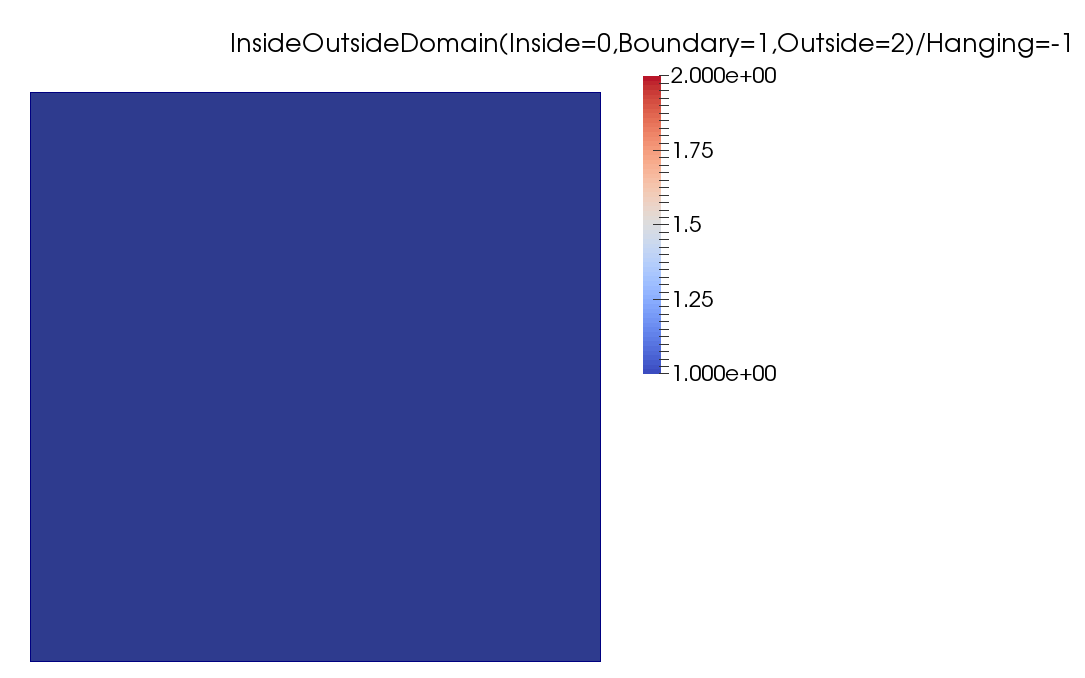
\includegraphics[width=0.8\textwidth]{10_quickstart/screenshot00.png}
\end{center}

\noindent
Congratulations: We have created the simplest adaptive Cartesian grid in 2d that
does exist. A single square!


\section{Some real AMR}

We now set up something slightly more complicated. 
First of all, we switch to a 3d setup rather than 2d. 
For this, open the makefile (\texttt{myproject/makefile}) and alter the
content of the \texttt{DIM} variable.

\begin{code}
# Set Dimension
# -------------
#DIM=-DDim2
DIM=-DDim3
#DIM=-DDim4
\end{code}

\noindent
If you clean your project (\texttt{make -f myproject/makefile clean}) and
rebuild your code, you see that the individual files are translated with the
compile switch 

\begin{code}
g++ ... -DDim3 ....
\end{code}

\noindent
Indeed, this is all that's required for Peano to run a 3d experiment rather than
a 2d setup. 

\begin{remark}
We do support currently up to 10-dimensional setups. If you require higher
dimensions, you might even be able to extend Peano accordingly by changing
solely the file \texttt{peano/utils/Dimensions.h}. But have fun with your memory
requirements exploding.
\end{remark}


Next, we will edit the file \texttt{myproject/mappings/CreateGrid.cpp}. 
Open it with your favourite text editor and search for the operation
\texttt{createBoundaryVertex}. 
Change it into the code below:


\begin{code}
void myproject::mappings::CreateGrid::createBoundaryVertex(
 myproject::Vertex&                          fineGridVertex,
 const tarch::la::Vector<DIMENSIONS,double>& fineGridX,
 const tarch::la::Vector<DIMENSIONS,double>& fineGridH,
 myproject::Vertex * const                   coarseGridVertices,
 const peano::grid::VertexEnumerator&     coarseGridVerticesEnumerator,
 myproject::Cell&                            coarseGridCell,
 const tarch::la::Vector<DIMENSIONS,int>&    fineGridPositionOfVertex
) {
  logTraceInWith6Arguments("createBoundaryVertex(...)", ...); 
    // leave this first line as it is
   
  if (coarseGridVerticesEnumerator.getLevel()<2) {
    fineGridVertex.refine();
  }

  logTraceOutWith1Argument("createBoundaryVertex(...)",fineGridVertex);
}
\end{code}


\noindent
If you compile this code and run the executable, you will (besides lots of
debug output) obtain a way bigger vtk file. 
If you visualise it this time, we observe that the code refines towards the
cube's boundary. 
You may want to play around with magic \texttt{2} in the operation above. 
Or you might want to continue to our final example.

\begin{center}
  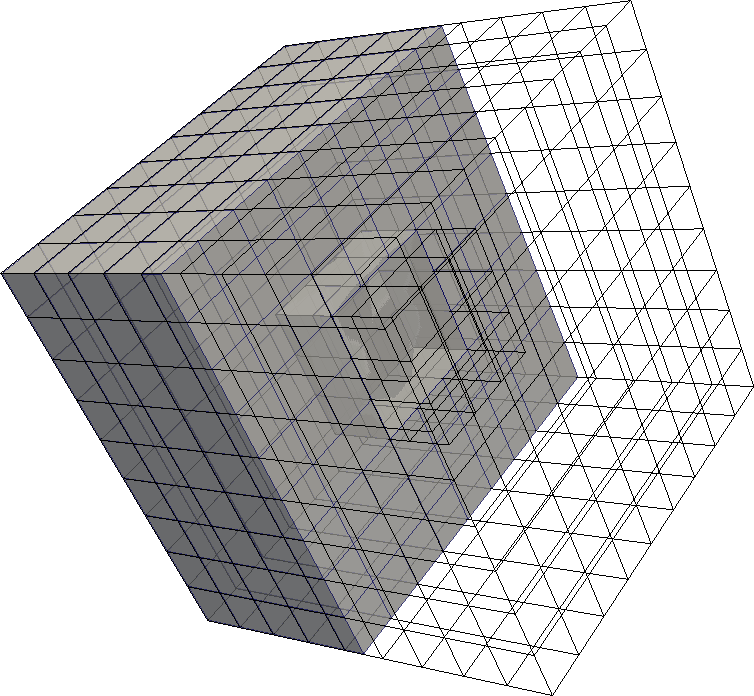
\includegraphics[width=0.55\textwidth]{10_quickstart/cube.png}
\end{center}


\section{A tree within the spacetree}

In the final example we create a slightly more interesting setup. 
We solely edit the operation \texttt{createInnerVertex} within the  
file \texttt{myproject/mappings/CreateGrid.cpp}, recompile it and 
have a look at the result.
When you study source code, please note the similarity to Matlab when we work
with vectors in Peano; as well as that the indices start with 0.
If your want to get rid of all the debug statements and are sick of long 
waiting times, remove the \texttt{-DDebug} statement in the line  
\texttt{PROJECT\_CFLAGS = -DDebug -DAsserts}
within the makefile.
There are more elegant ways to filter out log statements that we will discuss
later.


\begin{code}

void myproject::mappings::CreateGrid::createInnerVertex(
 myproject::Vertex&                          fineGridVertex,
 const tarch::la::Vector<DIMENSIONS,double>& fineGridX,
 const tarch::la::Vector<DIMENSIONS,double>& fineGridH,
 myproject::Vertex * const                   coarseGridVertices,
 const peano::grid::VertexEnumerator&      coarseGridVerticesEnumerator,
 myproject::Cell&                            coarseGridCell,
 const tarch::la::Vector<DIMENSIONS,int>&    fineGridPositionOfVertex 
) {
 logTraceInWith6Arguments("createInnerVertex(...)",fineGridVertex,...);
  
 if (
   fineGridVertex.getRefinementControl()==Vertex::Records::Unrefined 
   &&
   coarseGridVerticesEnumerator.getLevel()<4
 ) {
   bool trunk = (fineGridX(0)-0.5)*(fineGridX(0)-0.5)
              + (fineGridX(2)-0.5)*(fineGridX(2)-0.5)<0.008;
   bool treeTop = (fineGridX(0)-0.5)*(fineGridX(0)-0.5)
                + (fineGridX(1)-0.7)*(fineGridX(1)-0.7)
                + (fineGridX(2)-0.5)*(fineGridX(2)-0.5)<0.3*0.3;
   if (trunk | treeTop) {
     fineGridVertex.refine();
   }
 }

 logTraceOutWith1Argument("createInnerVertex(...)",fineGridVertex);
}
\end{code}

So here's what I get. Feel free to create better pics:

\begin{center}
  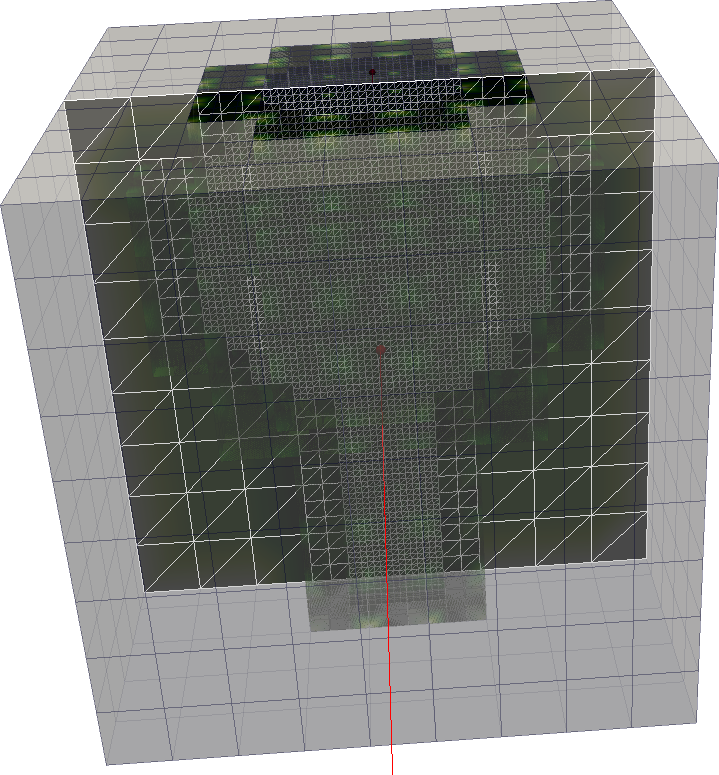
\includegraphics[width=0.55\textwidth]{10_quickstart/tree.png}
\end{center}




 
 \chapter{Basic Programming Course}
 \label{chapter:basics-explained}

 \chapter{Basic Programming Course}
\label{chapter:basics-explained}


\chapterDescription
  {
    15 minutes for the programming but perhaps around 30 minutes for the
    visualisation.
  }
  {
    Chapter \ref{chapter:quickstart}.
  }


In this section, we study a 2d example.
Please adopt your makefile accordingly.
Furthermore, we use the files \texttt{VTKMultilevelGridVisualiserHeader} and
\texttt{...Implementation} as well as
\texttt{VTK2dTreeVisualiser...}.
If you have downloaded the whole Peano repository, these files can be found in
\texttt{pdt/usrtemplates}.
If not, you have to download them manually from the webpage.
Please set up an empty project as discussed in Chapter
\ref{chapter:quickstart} and implement one operation as follows (all other
operations can remain empty/only filled with log statements):


\begin{code}
void myproject::mappings::CreateGrid::touchVertexLastTime(
      myproject::Vertex&               fineGridVertex,
      const tarch::la::Vector<DIMENSIONS,double>&                          fineGridX,
      const tarch::la::Vector<DIMENSIONS,double>&                          fineGridH,
      myproject::Vertex * const        coarseGridVertices,
      const peano::grid::VertexEnumerator&                coarseGridVerticesEnumerator,
      myproject::Cell&                 coarseGridCell,
      const tarch::la::Vector<DIMENSIONS,int>&                             fineGridPositionOfVertex
) {
  logTraceInWith6Arguments( "touchVertexFirstTime(...)", fineGridVertex, fineGridX, ...

  if (
    coarseGridVerticesEnumerator.getLevel()<5
    &&
    tarch::la::equals( fineGridX, 0.0 )
    &&
    fineGridVertex.getRefinementControl()==Vertex::Records::Unrefined
  ) {
    fineGridVertex.refine();
  }

  logTraceOutWith1Argument( "touchVertexFirstTime(...)", fineGridVertex );
}

\end{code}


\noindent
This source fragment requires some additional explanation. 
We neglect the enumerator stuff for the time being.
That will become clear later throughout the present chapter.
The refinement control check says `well, refine, but do it only on unrefined
vertices'.
It's just a matter of good style, not to call \texttt{refine} on a refined
vertex.
The middle line uses a function from the tarch's linear algebra namespace. 
It takes the \texttt{fineGridX} vector (the position of the vertex in space) and
checks whether all entries equal zero.
As we are working with floating point numbers, it is not a bit-wise check. 
Instead, it uses an interval of machine precision around zero.
You may want to change this notion of machine precision in Peano (file
\texttt{Scalar} within the \texttt{tarch::la} namespace). 
In general, it would be a good idea to study the content of the \texttt{la}
component soon---there's lots of useful stuff in there to work with
tiny, dense vectors\footnote{Peano someday should perhaps be rewritten to use
boost linear algebra or some fancy template library. Feel free to do so. Right
at the moment, it is all plain hand-craftet routines.}.

\begin{remark}
  Peano realises a {\bf vertex-based}, {\bf logical-or} refinement: You can
  invoke \texttt{refine} on any unrefined vertex. Peano then refines all cells
  around a vertex in the present or next traversal (it basically tries to do it
  asap, but sometimes data consistency constraints require it to postpone the
  actual refinement by one iteration). The other way round, you may read it as
  follows: A cell is refined if the refinement flag is set for any adjacent
  vertex.
\end{remark}


Whenever you use Peano, you have to do three things:
\begin{enumerate}
  \item Decide which algorithmic phases do exist and in which order they are
  called. Examples for algorithmic phases could be: set up grid, initialise all
  variables, refine regions of interest, perform an iterative solve step, plot
  some data, compute metrics on the solution, \ldots
  \item Model the data, i.e.~decide which data is assigned to the vertices and
  cells of the grid.
  \item Implement the different actions on this data model that are used by the
  algorithmic phases.
\end{enumerate}

This scheme lacks the bullet point `run through the grid'. 
Indeed, Peano applications do never run themselves through the spacetree.
They specify which set of operations is to be called throughout a run through
the grid, i.e.~they say what is done on which data.
Afterward, they invoke the iteration and leave it to Peano to run through the
grid and invoke these operations in the right order on the right ranks using all
the cores you have on your machine\footnote{This statements requires
explanation, and indeed it is not {\em that} straightforward. But the idea is
phrases correctly: the application codes specifies what is to be done and then
outsources the scheduling and the responsibility to use a multicore machine to
Peano.}.
This scheme realises something people call `The Hollywood Principle': Don't
call us, we call you!


\begin{remark}
  The {\bf inversion of control} is the fundamental difference of Peano to other
  spacetree-based codes offered as a library. 
  And typically it is the property many users first struggle with.
  Often, people claim `I have to run through the grid this and that way'. 
  Often, they are wrong.
  It can become quite comfortable to leave it to someone else to decide how 
  grid traversals are realised.
  And it allows the grid traversal in turn to optimise the code under the hook
  without an application developer to bother.
\end{remark}


\section{On the power of loosing control}

The algorithmic phases, i.e.~what can be done on a grid, are specified in the
specification file.
Open your project's file. 
There are two different parts of the document that are of interest to us:
An {\em event mapping} is an algorithmic step that you have to implement
yourself.
In this chapter's example, we want to do two things: create a grid and count all
the vertices. 
Furthermore, we want to plot our grid, but let's keep in mind that Peano has
some predefined actions as well.
So we augment our mapping set as follows:

\begin{code}
// Creates the grid
event-mapping:
  name: CreateGrid

// Counts all the vertices within the grid
event-mapping:
  name: CountVertices
\end{code}

\noindent
Event mappings cannot be used directly.
Instead, we have to specify adapters. 
Adapters take the tree traversal and invoke for each grid part a set of events. 
As we distinguish adapters which basically just glue together (multiple) events
from the events themselves, we will be able to do the following later:
we write a fancy visualisation routine, a routine that adopts the grid to a new
data set and some compute routines.
As we have done this in three different event sets, we can then combine these
events in various ways: compute something and at the same time plot, compute
only, plot and afterward adopt the grid, and so forth.
For the time being, we use the following adapters:

\begin{code}
adapter:
  name: CreateGrid
  merge-with-user-defined-mapping: CreateGrid

adapter:
  name: CountVertices
  merge-with-user-defined-mapping: CountVertices

adapter:
  name: CreateGridAndPlot
  merge-with-user-defined-mapping: CreateGrid
  merge-with-predefined-mapping: VTKGridVisualiser(finegrid)
  merge-with-predefined-mapping: VTKMultilevelGridVisualiser(grid)

adapter:
  name: CountVerticesAndPlot
  merge-with-user-defined-mapping: CountVertices
  merge-with-predefined-mapping: VTKMultilevelGridVisualiser(grid)

adapter:
  name: Plot
  merge-with-predefined-mapping: VTKGridVisualiser(finalgrid)
\end{code}

The first two adapters are trivial: 
They basically delegate to one event set. 
The next two take one event set each and invoke it. 
Furthermore, they also use a predefined event set. 
They will call \texttt{CreateGrid} or \texttt{CountVertices}, respectively, and
at the same time plot.
If you create all code with 

\begin{code}
java -jar <mypath>/pdt.jar --generate-gluecode
myproject/project.peano-specification myproject <mypath>/usrtemplates
\end{code}

\noindent
it is the directory \texttt{usrtemplate} where the PDT searches for the
predefined event sets.
The last adapter by the way is a trivil one, too: It invokes only one of the
events that ship with Peano.


Next, please create all glue code and have a quick look into the file
\texttt{runners/Runner.cpp}.
This file is the starting point of Peano.
The C++ main routine does some setup steps and then creates an instance of the
Runner (see the source code yourself if you don't believe).
It then invokes \texttt{run()} which in turn continues to \texttt{runAsMaster}
or \texttt{runAsWorker()}.
The latter will play a role once we use MPI.
For the time being, let's focus on the master's routine.
Here, we see the following:

\begin{code}
int myproject::runners::Runner::runAsMaster(myproject::repositories::Repository& repository) {
  peano::utils::UserInterface userInterface;
  userInterface.writeHeader();

  // @todo Insert your code here
  
  // Start of dummy implementation
  
  repository.switchToCreateGrid(); repository.iterate();
  repository.switchToCountVertices(); repository.iterate();
  repository.switchToCreateGridAndPlot(); repository.iterate();
  repository.switchToCountVerticesAndPlot(); repository.iterate();
  repository.switchToPlot(); repository.iterate();

 
 
  repository.logIterationStatistics();
  repository.terminate();
  // End of dummy implementation

  return 0;
}
\end{code}

The PDT cannot know what exactly we do, so it basically runs all the adapters we
have specified.
This is the place where we implement our overall algorithm, i.e.~the big
picture.
Lets change it as follows:

\begin{code}
  peano::utils::UserInterface userInterface;
  userInterface.writeHeader();

  repository.switchToCreateGridAndPlot();
  for (int i=0; i<10; i++) repository.iterate();
  repository.switchToCountVertices(); repository.iterate();

  repository.logIterationStatistics();
  repository.terminate();

  return 0;
\end{code}

\noindent
This algorithm says that we want to create a grid and at the same time plot it.
We want to do this ten times in a row.
Afterward, we switch to our vertex counting and want to run through the grid
once more. 
This time, nothing shall be plotted.
We just want to know how many vertices there are.


We really do not care about how the code runs through the grid.
We also do not really care how all vertices, cells, whatever are processed.
We say what is done in which order from a bird eye's perspective.
If you compile the code and run it now, you should end up with a sequence of vtk
files. 
You might want to make a video (take the files that are called
\texttt{finegrid-}something).
Below are some screenshots:


\begin{center}
  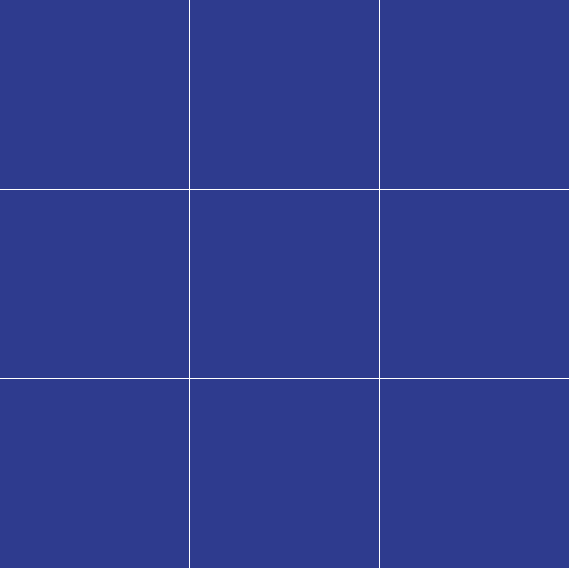
\includegraphics[width=0.3\textwidth]{11_basics/grid00.png}
  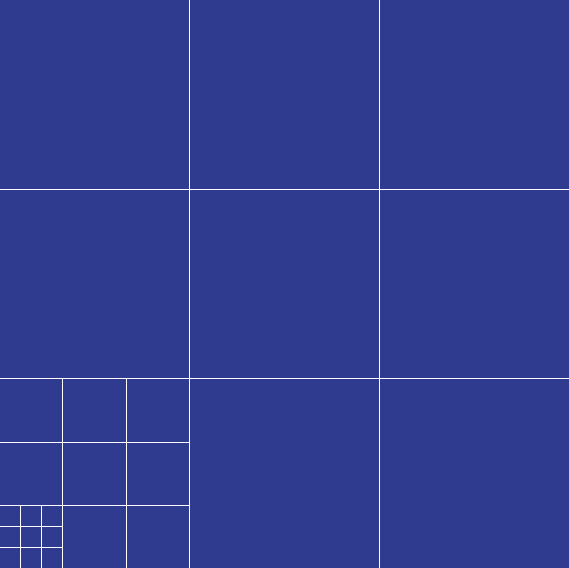
\includegraphics[width=0.3\textwidth]{11_basics/grid01.png}
  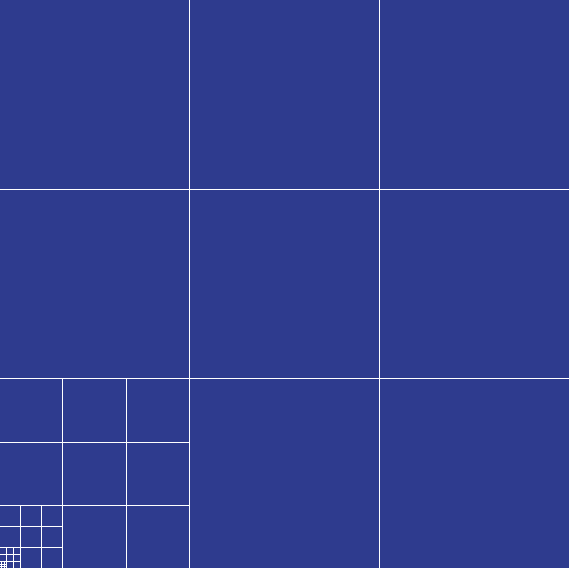
\includegraphics[width=0.3\textwidth]{11_basics/grid02.png}
\end{center}


\section{What happens}


\begin{center}
  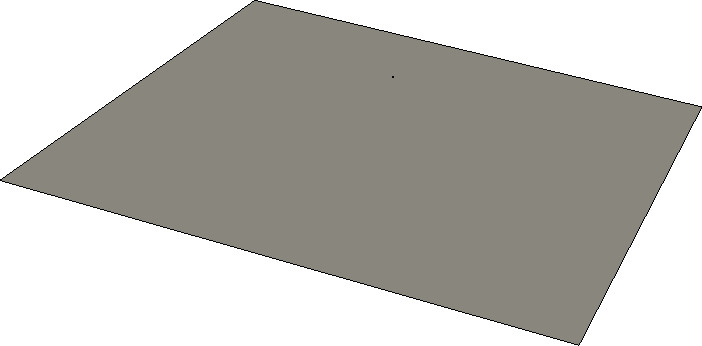
\includegraphics[width=0.45\textwidth]{11_basics/construction00.png}
  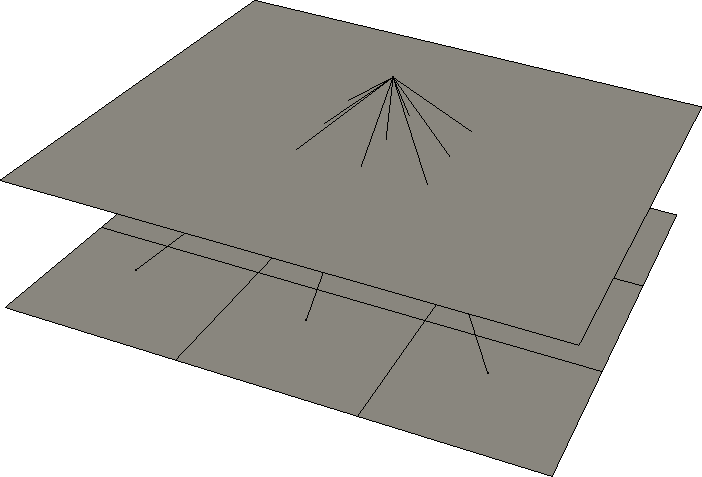
\includegraphics[width=0.45\textwidth]{11_basics/construction01.png}
  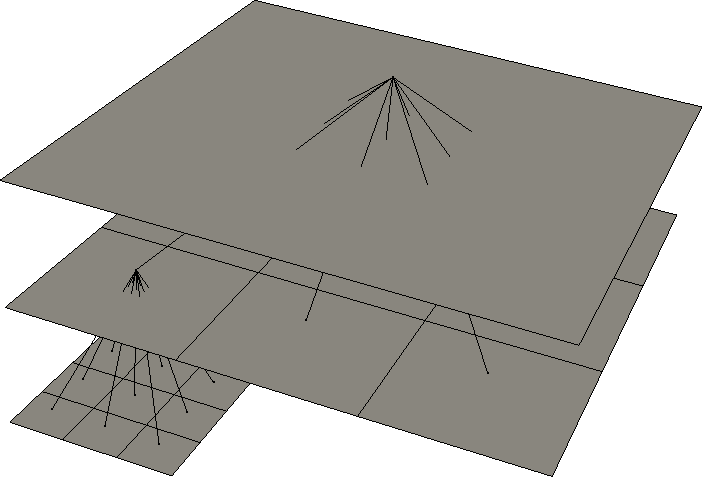
\includegraphics[width=0.45\textwidth]{11_basics/construction02.png}
  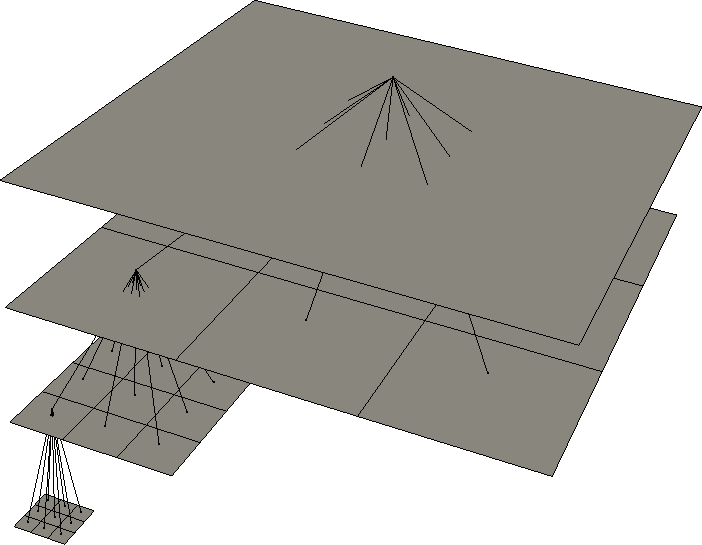
\includegraphics[width=0.45\textwidth]{11_basics/construction03.png}
\end{center}

% UserInterface interpretieren
% Welche events sind da
% was passiert
% Log lesen
% 
% 



\section{Data model}
Prior to a discussion of Peano's data model, it might make sense to load all the
files \texttt{grid-level-?-0.vtk} into your favourite visualisation software.
Dilate them according to their level encoded in the name.
In Paraview, you have to select each file, apply
Filters/Alphabetical/Transform, and dilate each file by -0.2 along the z-axis
per level.
You might end up with something alike:



\begin{center}
  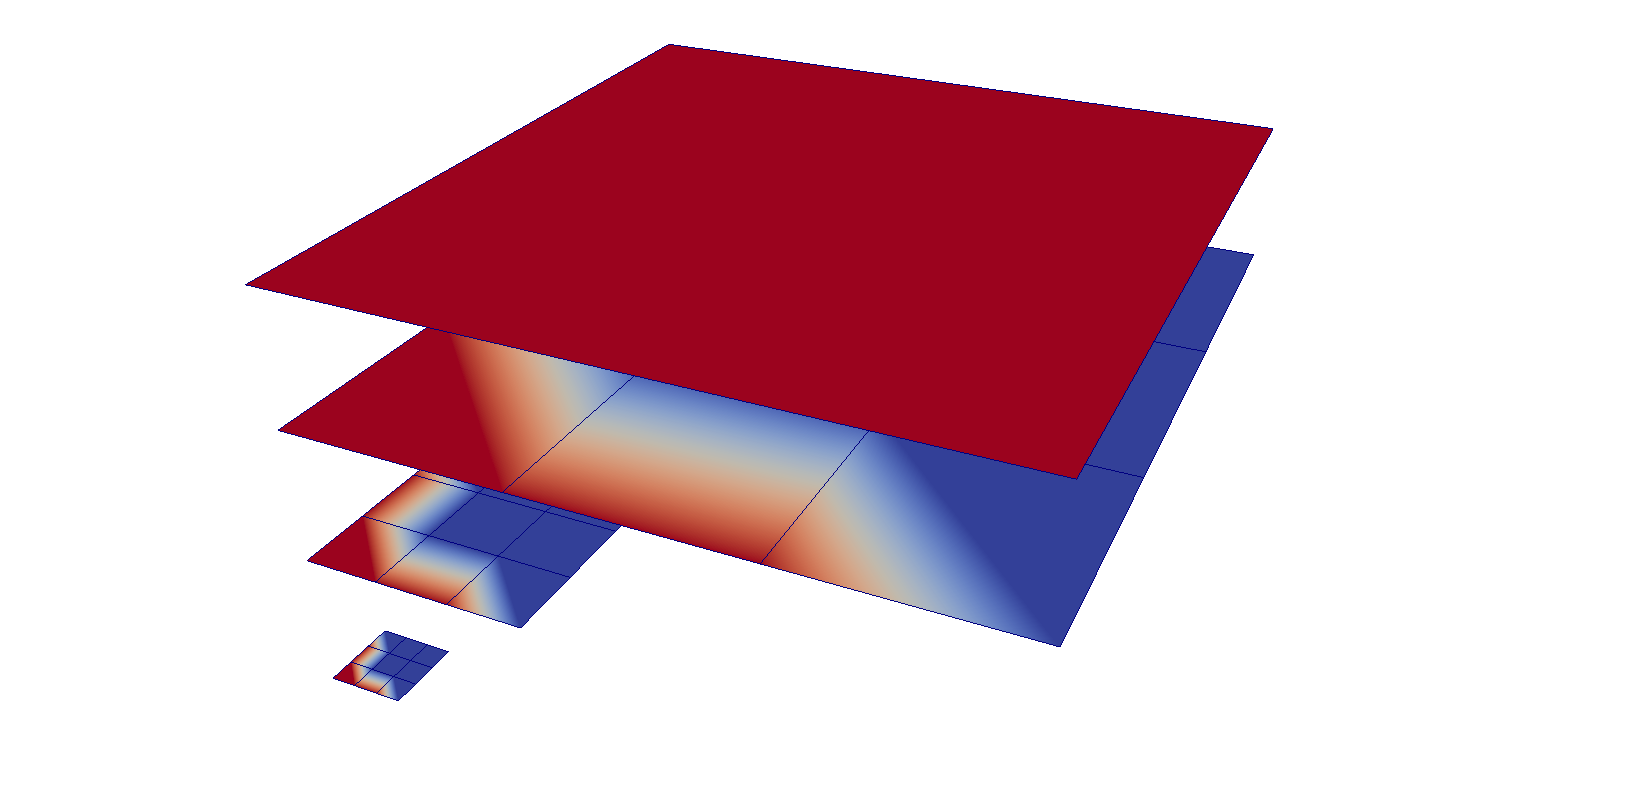
\includegraphics[width=0.8\textwidth]{11_basics/tree00.png}
\end{center}

\noindent
Again, feel free to create a video that shows how additional levels are added in
each step.
There's a more elegant way to end up with a similar picture. 
I once created a graph visualiser that is today also available as predefined
mapping. Just modify your adapters as follows:

\begin{code}
adapter:
  name: CreateGridAndPlot
  merge-with-user-defined-mapping: CreateGrid
  merge-with-predefined-mapping: VTK2dTreeVisualiser(tree,getLevel)
\end{code}

\noindent
This time, creating a video should be straightforward.
\begin{center}
  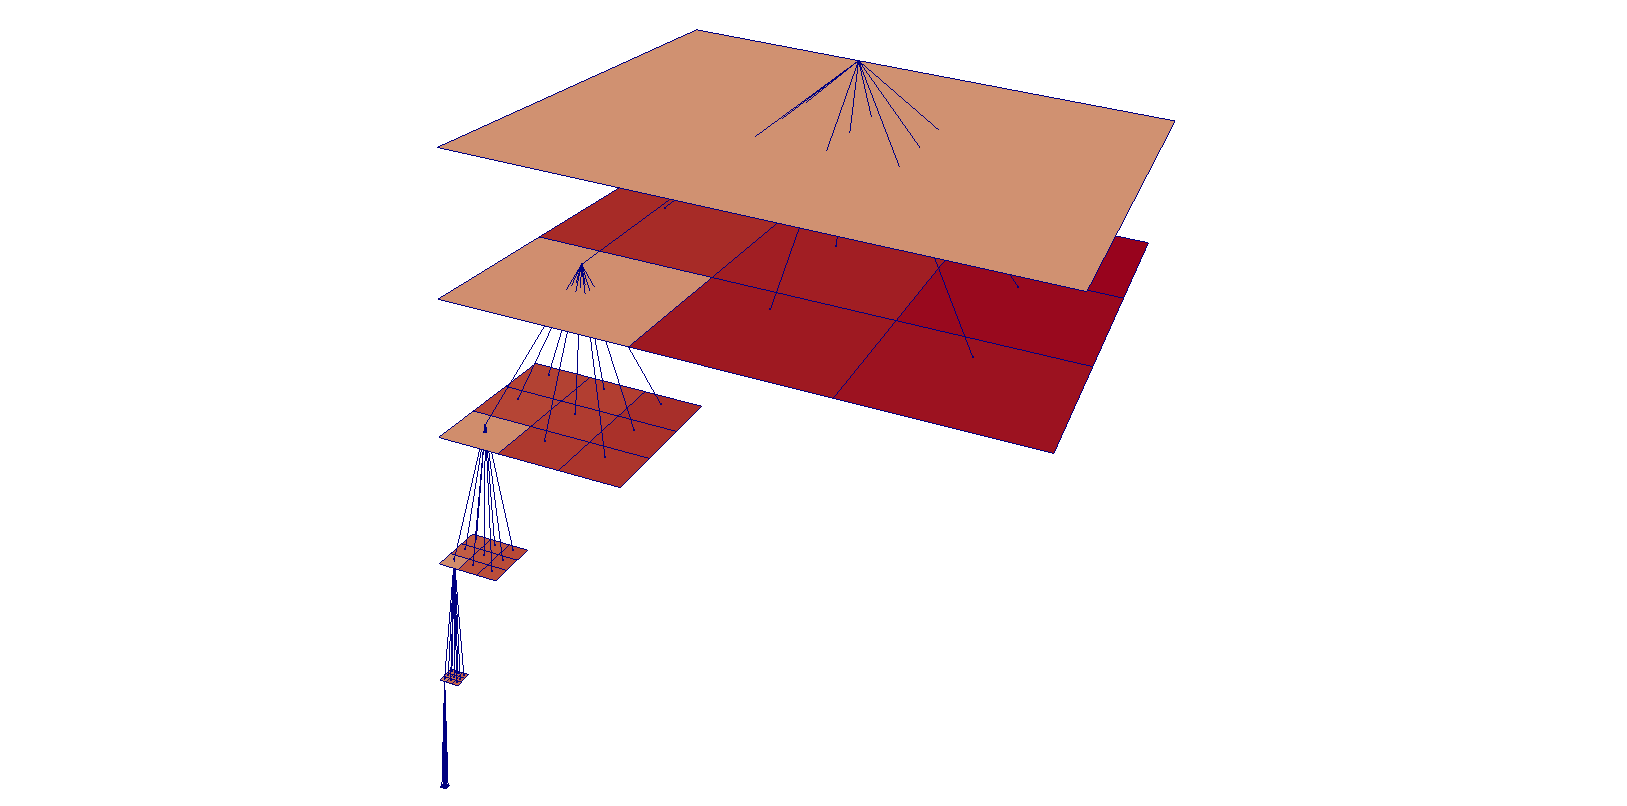
\includegraphics[width=0.8\textwidth]{11_basics/tree01.png}
\end{center}

% Data Model
% Visualisierung von Einbettung
% Wo liegen welche Daten
% 
% Remark: How to realise degrees of freedom associated to faces or edges
% 


\section{Counting vertices}
% We could use the repository's operations
% Do it yourself and then compare
% Finale: Vertices zaehlen
% Den Wert von einem double umsetzen



 \section{Logging, statistics, assertions}
\label{section:logging}

\subsection{The user interface}

\subsection{Repository fields}

\subsection{Log filter}

\subsection{Using logging and tracing}

\subsection{Statistics}

% Hier gleich das Python-Script einfuehren.

\subsection{Assertions}



% vertex enumerator
 \section{DaStGen primer and the heap}
\label{section:dastgen-and-heap}




So what we might do now is the following. Open the \texttt{Cell.def} and edit it
accordingly. 
Rerun the PDT, recompile, and work.


\begin{code}
Packed-Type: short int;


class myproject::dastgen::Cell {
  discard    parallelise int     myNonPersistentInteger;
  persistent parallelise double  myValue;
  persistent parallelise bool    myBool1;
  persistent parallelise bool    myBool2;
};
\end{code}


 \section{Filling the element-wise traversal with life}

% Element-wise traversal.
% Wo liegen welche Daten
% Enumerator
% Wer aggregiert was
% 
% Remark: How to realise degrees of freedom associated to faces or edges
% 




% We could use the repository's operations
% Do it yourself and then compare
% Finale: Vertices zaehlen
% Den Wert von einem double umsetzen








 \chapter{Applications}
 \label{chapter:application}

 \section{Patch-based solvers}


\chapterDescription
  {
    60 minutes.
  }
  {
    Chapter \ref{chapter:quickstart}.
  }

In this section, we sketch how to realise a simple explicit heat equation
solver that is based upon patches.
The idea is that we embed a small regular Cartesian grid into each individual
spacetree leaf.
This patch is surrounded by a halo/ghost cell layer holding copies from
neighbouring patches.

\begin{center}
  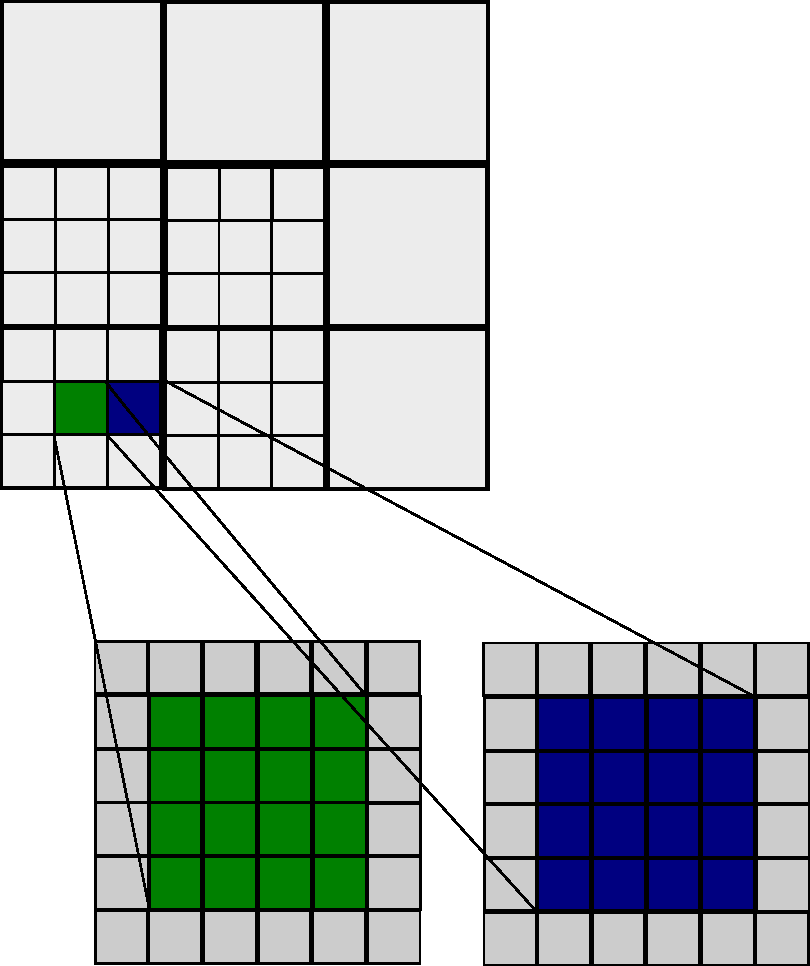
\includegraphics[width=0.4\textwidth]{22_patch-based-solver/patches.pdf}
\end{center}

In the sketch, we enbed $4\times 4$ patches into the spacetree cells.
Two cells (blue and green) are illustrated.
Each patch is surrounded by a halo layer of size one.
We will write the code to work within the patches, while the layers around the
patches will hold copies of the neighbouring patches and thus couple them.

For this endeavour, we need the toolbox \texttt{multiscalelinkedcell} that you
can download from the Peano webpage.
We assume that the whole toolbox is unzipped into a directory
\texttt{multiscalelinkedcell} which is held by your source directory.


\subsection{Preparation}

We start with the creation of a file \texttt{PatchDescription.def} in your
project's root directory. 
In our example, each patch solely shall hold one array of unknowns $u$ that are
associated to the vertices of the patch.
So each patch will have exactly $(4+2+1)^2$ unknowns (the four is the size,
there's two halo cells along each coordinate axis, and then there's finally one
more vertex than there are cells).
Besides the unknowns called $u$, we also store the position and size as well as
the level with each patch---well-aware that level and size are kind of
redundant.

\begin{code}
#include "peano/utils/Globals.h"

Packed-Type:  int;

Constant: DIMENSIONS;

/**
 * A cell description describes one individual patch of the overall grid, i.e. 
 * it holds pointers to the actual data of the patch (arrays) and its meta data
 * such as time stamps. Each unrefined node of the spacetree, i.e. each leaf, 
 * holds exactly one instance of this class. 
 */
class myprojectname::records::PatchDescription {
  /**
   * Two pointers to float arrays.
   */
  parallelise persistent int     u;
  /**
   * I need level and offset to be able to determine the source and image in 
   * the adaptive case.
   */
  parallelise persistent int     level;
  parallelise persistent double  offset[DIMENSIONS];
  parallelise persistent double  size[DIMENSIONS];
};
\end{code}

Please note that $u$ is modelled as integer. 
Actually, we do not hold the data directly within the patch description but we
make the patch description hold a pointer to the actual data.
The data will be managed by Peano on the heap. 
The heap uses integers as pointers.
They are actually hash map indices.


Our system design is as follows:
\begin{itemize}
  \item Each cell holds a pointer to one \texttt{PatchDescription}.
  \item The \texttt{PatchDescription} holds a pointer to the actual patch data
  and comprises some additional meta data (such as the level).
  \item Each vertex holds $2^d$ pointers to the
  \texttt{PatchDescription} instances belonging to the adjacent cells.
\end{itemize}


Whenever we enter a cell, we can thus take its patch description, and get the
actual data from this description.
Alternatively, we can use the cell's $2^d$ adjacent vertices. 
As they know the adjacent patch descriptions, we can also get the data
associated to cell neighbours and thus befil the ghost layers, e.g.


Take the Peano description file of our project ensurte that it contains the
following lines:
\begin{code}
heap-dastgen-file: PatchDescription.def

[...]

vertex:
  dastgen-file: Vertex.def
  read vector2PowD(int): PatchIndex
  write vector2PowD(int): PatchIndex
  
[...]

event-mapping:
  name: Mapping1


event-mapping:
  name: Mapping2
  
[...]

adapter:
  name: Adapter1
  merge-with-user-defined-mapping: Mapping1
  merge-with-predefined-mapping: MultiscaleLinkedCell(PatchIndex)

adapter:
  name: Adapter2
  merge-with-user-defined-mapping: Mapping2
  merge-with-predefined-mapping: MultiscaleLinkedCell(PatchIndex)
\end{code}

Managing all the adjaceny data (making each vertex point to the right patch)
obviously is a tedious task.
The \texttt{multiscalelinkedcell} toolbox fortunately does most of the stuff for
us, if we augment each adapter with a predefined mapping, tell this mapping what
the attribute for the patch handling will be (\texttt{PatchIndex}), and augment
the vertex accordingly. 
Finally, open \texttt{Vertex.def} and augment it accordingly:

\begin{code}
#include "peano/utils/Globals.h"

Packed-Type:  int;

Constant: TWO_POWER_D;

class myprojectname::dastgen::Vertex {
  /**
   * These guys are pointers to the adjacent cells. Actually, they do not point 
   * to the neighbouring cells but to the heap indices associated to these cells.
   * These heap indices reference one or several instances of PatchDescription.
   */
  expose persistent int patchIndex[TWO_POWER_D];  
  
  [...]
};
\end{code}

We run the translation process and add the toolbox directory to the PDT call:
\begin{code}
 java -jar <mypath>/pdt.jar <mypath>/project.peano-specification <mypath> \
 <mypath>/usrtemplates:<mypath>/multiscalelinkedcell
\end{code}


The PDT in collaboration with the toolbox will now create code that makes each
vertex track the \texttt{patchIndex} value of the adjacent cells.
If you change your grid, the indices are updated automatically, as long as you
merge \texttt{MultiscaleLinkedCell} into your adapters.
To make the code compile, you finally have to add a routine 
\begin{code}
  int getPatchIndex() const;
\end{code}
to your Cell class. 
Make the routine return the value of an attribute \texttt{persistent int 
patchIndex} that you add to your \texttt{Cell.def}.
Set this field to -1 in the default constructor.

\subsection{Setting up the patches}

Before we start any coding, we have to specify which heaps we want to use to
administer the patch description objects and the actual $u$ data.
One option is to define this centrally in the \texttt{Cell.h} file that is
generated by the PDT:
\begin{code}
#include "peano/heap/Heap.h"
#include "<mypath>/records/PatchDescription.h"

namespace myprojectsnamespace { 
  class Cell;
  
  typedef peano::heap::PlainHeap< myprojectsnamespace::records::PatchDescription >  
    PatchDescriptionHeap;
  typedef peano::heap::PlainDoubleHeap                                    DataHeap;
}
\end{code}

\noindent
In this setup, we use the plain heap from Peano's heap directory to administer
both the data and the patch descriptions. 
There are several other, more sophisticated, heap implementations available. 
While they allow you to tune your code for special purposes, the plain heap
typically is a good starting point.

To set up the patches, we create plug into the mapping creating our grid. 
Alternatively, we can first create the grid and then outsource the patch
initialisation into an additional mapping.
In any case, I strongly encourage you to initialise the heap as a first step. 
This is however optional: 
\begin{code}
void myprojectsnamespace::mappings::InitPatches::beginIteration(
  ...
) {
  logTraceInWith1Argument( "beginIteration(State)", solverState );

  PatchDescriptionHeap::getInstance().setName( "patch-description-heap" );
  DataHeap::getInstance().setName( "data-heap" );

  logTraceOutWith1Argument( "beginIteration(State)", solverState);
}
\end{code}
So far, each cell points to index -1 as patch description index, and each vertex
knows that all adjacent cells point to -1. We change this now as we plug into 
\texttt{enterCell} and introduce a new operation in Cell:

\begin{code}
void myprojectsnamespace::mappings::InitPatches::enterCell(
  ...
) {
  fineGridCell.init( ... ); // please pass through the level, the offset and the size
}


void myprojectsnamespace::Cell::initCellInComputeTree( ... ) {
  const int newPatchIndex = PatchDescriptionHeap::getInstance().createData(1);
  _cellData.setPatchIndex( newPatchIndex );
  assertion( newPatchIndex>=0 );
  ...
}

\end{code}

\noindent
We finally befill the patch data, i.e.~replace the dots in
\texttt{initCellInComputeTree}.
This is a three-fold process.
First, we initialise all the meta data.
Second, we create the real patch. 
Finally, we make the meta data record point to this data, while 
the cell itself points to the \texttt{PatchDescription} instance.
 
\begin{center}
  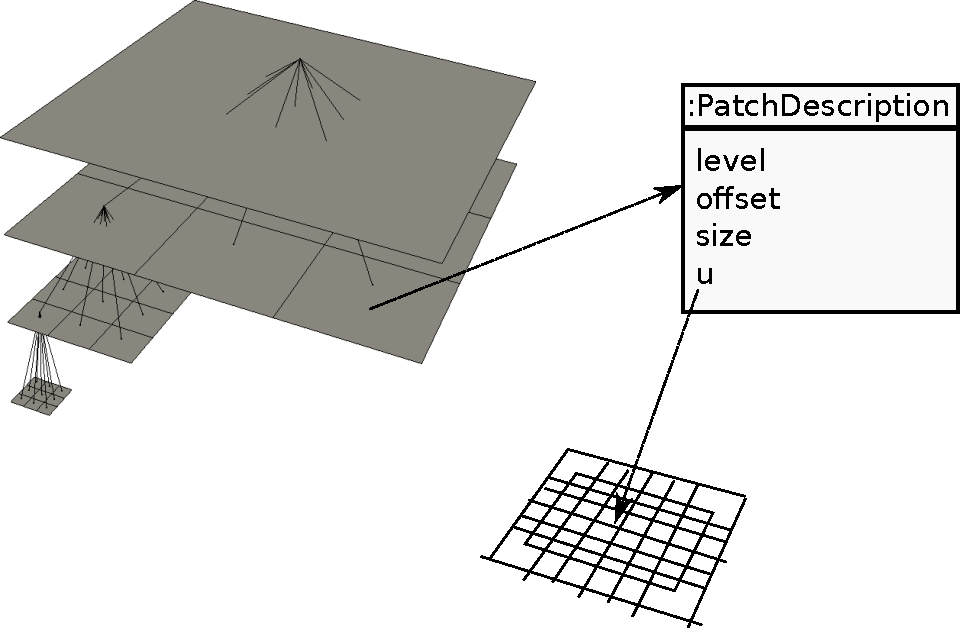
\includegraphics[width=0.5\textwidth]{22_patch-based-solver/data.pdf}
\end{center}

\noindent
It is up to you to specificy the semantics of the data arrays used. 
They can represent overlapping or non-overlapping patches.
It just has paid off not to make any overlap exceed any neighbouring cell on the
same level.
The introductory sketch of this chapter illustrates $4\times 4$ patches with a
ghost layer/overlap of one. 
A code for this setup might read as follows:

\begin{code}
void myprojectsnamespace::Cell::initCellInComputeTree( ... ) {
  const int numberOfPatchDescriptionsPerCell = 1;
  const int newPatchIndex = PatchDescriptionHeap::getInstance().createData
    (numberOfPatchDescriptionsPerCell);
  _cellData.setPatchIndex( newPatchIndex );
  assertion( newPatchIndex>=0 );

  records::PatchDescription patchDescription =
    PatchDescriptionHeap::getInstance().getData(newPatchIndex)[0]; 
  
  patchDescription.setU( DataHeap::getInstance().createData(7*7) );
  patchDescription.setLevel(...);
  patchDescription.setOffset(...);
  patchDescription.setSize(...);
}

\end{code}


\begin{remark}
  There is absolutely no reason to restrict a code to use only the finest level
  of the spacetree. Furthermore, it might make sense to use different patch
  sizes in different cells of the same level. Please note that all the patch
  techniques also work if you store higher order DG shape functions in your
  cells, e.g.
\end{remark}



\subsection{Working with patches on regular grids}

As each cell points to patch description through its field \texttt{PatchIndex},
it is a natural choice to work with the associated patch data in
\texttt{enterCell}.
Before we actually do the work, we use the data from the 
\texttt{PatchIndex} objects of the neighbouring cells to initialise our ghost
cells.
In our case, a simple copying does the job. In other situations, you might have
to implement more sophisticated projection operators.

\begin{code}
#include "multiscalelinkedcell/HangingVertexBookkeeper.h"
#include "multiscalelinkedcell/SAMRTools.h"
#include "peano/utils/Loop.h"
...
void pesplines::mappings::JacobiUpdate::enterCell( ... ) {
 if (
  !fineGridCell.isRefined()
  &&
  multiscalelinkedcell::HangingVertexBookkeeper::allAdjacencyInformationIsAvailable(
   VertexOperations::readPatchIndex(fineGridVerticesEnumerator,fineGridVertices)
  )
 ) {
  intialiseGhostLayerOfPatch(
    fineGridCell,
    fineGridVertices,
    fineGridVerticesEnumerator
  );
   
  solve(
    PatchDescriptionHeap::getInstance().getData( fineGridCell.getPatchIndex() )[0],
    fineGridVerticesEnumerator.getCellSize()
  );
 }  
}
\end{code}

\noindent
The use of the predicate \texttt{allAdjacencyInformationIsAvailable} is too
careful here: it should always return \texttt{true}.
In dynamically adaptive settings, it can happen that adjacency information in
the vertices (i.e.~which patch descriptions are held by the adjacent cells) it
not up-to-date immediately.
In such a case, the branching would skip a cell with incomplete data and wait
for the next traversal where all information is available.


The initialisation of the ghost layer uses Peano's d-dimensional loops (the
code then should work for $d=3$ as well), it rather technical, but not too
difficult to understand as it realises plain copying at the end of the day.
Again, we use operations provided by the \texttt{multiscalelinkedcell} package:

\begin{code}
void pesplines::mappings::MatVec::intialiseGhostLayerOfCell(
 Cell&                                 fineGridCell,
 Vertex * const                        fineGridVertices,
 const peano::grid::VertexEnumerator&  fineGridVerticesEnumerator
) {
 const tarch::la::Vector<THREE_POWER_D,int> neighbourCellIndices = 
  multiscalelinkedcell::getIndicesAroundCell(
   VertexOperations::readPatchIndex(fineGridVerticesEnumerator,fineGridVertices)
 );

 assertion3(
   multiscalelinkedcell::HangingVertexBookkeeper::allAdjacencyInformationIsAvailable(
    VertexOperations::readPatchIndex(fineGridVerticesEnumerator,fineGridVertices)
   ),
   fineGridVerticesEnumerator.toString(),
   VertexOperations::readPatchIndex(fineGridVerticesEnumerator,fineGridVertices),
   neighbourCellIndices
 ); // no enty of neighbourCellIndices points to a patch description on the
    // heap that does not exist
 
 // we take data from surrounding patches and always write into the
 // patch in the center (destPatchDescription)
 records::PatchDescription& destPatchDescription = 
  PatchDescriptionHeap::getInstance().getData( fineGridCell.getPatchIndex())[0];

 dfor3(i)
  // i does not point to the central patch (all entries 1) and is valid
  // i.e. we are not at the domain boundary, e.g.
  if (
   i!=tarch::la::Vector<DIMENSIONS,int>(1) &&
   neighbourCellIndices(iScalar) > 
    multiscalelinkedcell::HangingVertexBookkeeper::InvalidAdjacencyIndex
  ) {
   assertion(neighbourCellIndices(iScalar)>=0);
   records::PatchDescription& srcPatchDescription 
    = PatchDescriptionHeap::getInstance().getData( neighbourCellIndices(iScalar) )[0];
 
   // this if is always true as long as we work with a regular grid
   if (srcPatchDescription.getLevel()==destPatchDescription.getLevel()) {
    // so now write your well-suited for loop here that befill all entries 
    // of the ghost layer of your patch. If the for loop determines the 
    // indices destVertexIndex and srcVertexIndex specifying vertices within 
    // the patch, then the loop body copying the data around reads as 
    DataHeap::getInstance().getData(destPatchDescription.getU())
      [destVertexIndex]._persistentRecords._u =
     DataHeap::getInstance().getData(srcPatchDescription.getU())
      [srcVertexIndex]._persistentRecords._u;
   }
  }
 enddforx // counterpart of dfor3 (see documentation in source code)
}
\end{code}

\noindent
The texttt{dfor3(i)} runs over a $\{0,1,2\}^d$ domain.
In the loop body (that has to be terminated by a \texttt{enddforx} pragma), it
provides two loop counters: \texttt{i} is a d-dimensional integer vector where
each entry is from $\{0,1,2\}$.
Furthermore, it gives us another loop counter \texttt{iScalar} which runs from 0
through $3^d-1$, i.e.~is a linearisation of \texttt{i}.
All the macros are defined in \texttt{Loop.h}.


\texttt{getIndicesAroundCell} is a helper function that takes the $2^d$ adjacent
vertices of a cell.
It actually requires their \texttt{PatchIndex} entries which are automatically
set by the predefined mapping.
The helper tool returns an array with $3^d$ entries to be read as a $3^d$
integer field.
The first entry holds the patch index of the left bottom neighbour.
The second entry holds the patch index of the bottom neighbour.
The fourth entry holds the patch index of the left neighbour.
The fifth entry hold the patch index of the cell itself.
And so forth.
The operation works for any dimension.
Study its source code documentation for details.


How the actual copying is done depends on the semantics of your data. 
It also depends on column-major or row-major storage formats for the patch data.
The implementation of the actual \texttt{solve} operation then finally is
straightforward: take the $u$-array and run through it. Again, a \texttt{dfor}
loop might simplify your code.
If you struggle with the \texttt{solve} operation, it might make sense to study
the plotting in the next section first. 
It uses exactly the sketched loop of the patch entries.


\subsection{Plotting}

We briefly sketch what rapid coding of the plotting of a patch-based solver
might look like.
For this, we rely on a mapping \texttt{Plot} that holds plotter classes from 
Peano's plotter component.


\begin{code}
#include "tarch/plotter/griddata/blockstructured/PatchWriterUnstructured.h"

namespace pesplines {
  namespace mappings {
    class Plot;
  }
}

class pesplines::mappings::Plot {
  private:
    ...
    static int                  _snapshotCounter;

    tarch::plotter::griddata::blockstructured::PatchWriter*                      _writer;
    tarch::plotter::griddata::blockstructured::PatchWriter::SinglePatchWriter*   _patchWriter;
    tarch::plotter::griddata::blockstructured::PatchWriter::VertexDataWriter*    _uWriter;
};
\end{code}

\noindent
The implementation plugs into \texttt{beginIteration} and \texttt{endIteration}
to open the plotter or to write its data into a file, respectively.
Depending on the build type, we either plot binary data or we plot a plain text
file that is easier to debug.

\begin{code}
int ...::mappings::Plot::_snapshotCounter(0);

void ...::mappings::Plot::beginIteration(
  ...::State&  solverState
) {
  #if defined(Asserts) || defined(Debug)
  _writer = new tarch::plotter::griddata::blockstructured::PatchWriterUnstructured( 
    new tarch::plotter::griddata::unstructured::vtk::VTKTextFileWriter() );
  #else
  _writer = new tarch::plotter::griddata::blockstructured::PatchWriterUnstructured( 
    new tarch::plotter::griddata::unstructured::vtk::VTKBinaryFileWriter() );
  #endif
  _patchWriter            = _writer->createSinglePatchWriter();

  _uWriter         = _writer->createVertexDataWriter("u",3);
}


void ...::mappings::Plot::endIteration(
  ...::State&  solverState
) {
  _patchWriter->close();
  _uWriter->close();

  delete _uWriter;
  delete _patchWriter;

  _uWriter = 0;
  _patchWriter = 0;

  std::ostringstream snapshotFileName;
  snapshotFileName << "solution"
                   #ifdef Parallel
                   << "-rank-" << tarch::parallel::Node::getInstance().getRank()
                   #endif
                   << "-" << _snapshotCounter
                   << ".vtk";
  _writer->writeToFile( snapshotFileName.str() );

  _snapshotCounter++;

  delete _writer;
  _writer = 0;
}
\end{code}

\noindent
The heart of the plotting can be found in \texttt{enterCell} where the
actual patch data it piped into the solution plotter:


\begin{code}
void ...::mappings::Plot::leaveCell(...) {
 if ( !fineGridCell.isRefined() ) {
  assertion(PatchDescriptionHeap::getInstance().isValidIndex(fineGridCell.getPatchIndex()));
  const records::PatchDescription& patchDescription   
   = PatchDescriptionHeap::getInstance().getData( fineGridCell.getPatchIndex() )[0];

  const std::pair<int,int> indexPair = _patchWriter->plotPatch(
    fineGridVerticesEnumerator.getVertexPosition(),
    fineGridVerticesEnumerator.getCellSize(),
    4+1 // number of inner cells per spacetree leaf
  );

  int unknownVertexIndex = indexPair.first;
  //int unknownCellIndex   = indexPair.second;

  dfor(i,4+1) {
   const tarch::la::Vector<DIMENSIONS,int> currentVertex = i + 1;
   const int linearisedCurrentVertex 
    = peano::utils::dLinearisedWithoutLookup(currentVertex,4+1);
   const double u = DataHeap::getInstance().getData(patchDescription.getU())
    [linearisedCurrentVertex]._persistentRecords._u;

    _uWriter->plotVertex( unknownVertexIndex,u );
    unknownVertexIndex++;
  }
 }
}
\end{code}



\subsection{Adaptive grids}


%  \section{Matrix-free Jacobi solver}
%  \section{Shallow water code}
%  \section{Molecular dynamics}
 
  \chapter{High Performance Computing}
  \section{MPI}

% pdfor. pfor

  \chapter{Tuning}
  \label{chapter:tuning}

  \section{Performance analysis}


\chapterDescription
  {
    Less than 10 minutes unless you postprocess a big file.
  }
  {
    You may work with the plain output that Peano writes to the terminal. If you
    use log filters (cmp.~Chapter \ref{chapter:logging}), it is important that
    you know how to switch particular logging infos on. You also need a working
    Python installation.
  }

\noindent
Prior to any parallelisation or tuning discussion, I want to emphasise that it
usually makes sense first of all to have a how Peano is performing from a grid
point of view. For this, the framework comes along with a rather useful script.

\begin{itemize}
  \item Run your code and ensure that \texttt{info} outputs from the
    \texttt{peano::performanceanalysis} component are enabled.
  \item Pipe the output into a file:
    \begin{code}
> ./myExecutable myArguments > outputfile.txt
    \end{code} 
    We call this file \texttt{outputfile.txt} from hereon.
  \item Pass the output file to Peano's performance analysis script written in
  Python. Besides the script (name), you also have to tell the script how many 
    MPI ranks you have used and how many threads have been enabled. Skip
    the arguments if you haven't used MPI.
    \begin{code}
> python <mypath>/peano/performanceanalysis/performanceanalysis.py outputfile.txt
    \end{code} 
  \item Open the web browser of your choice and open the file
  \texttt{outputfile.txt.html}
\end{itemize}

\begin{remark}
Besides the output written by Peano through the component
\texttt{peano::performanceanalysis}, you also have to use the
\texttt{CommandLineLogger} (the default), and you have to make this one write
out time stamps as well as trace information. If you use your own logger or a
modified log format, the Python script will fail.
\end{remark}

If you browse through your directory, you will notice that all graphs are
written both as png and as pdf. 
You can thus integrate them directly into your \LaTeX\ reports.

  \section{Reducing the MPI grid setup and initial load balancing overhead}


\chapterDescription
  {
    Around 30 minutes.
  }
  {
    A working MPI code.
  }


In this section, we assume that you've a reasonable load balancing and that you
were able to postprocess your performance analysis outputs. We discuss 


\paragraph{The smell}

\begin{center}
  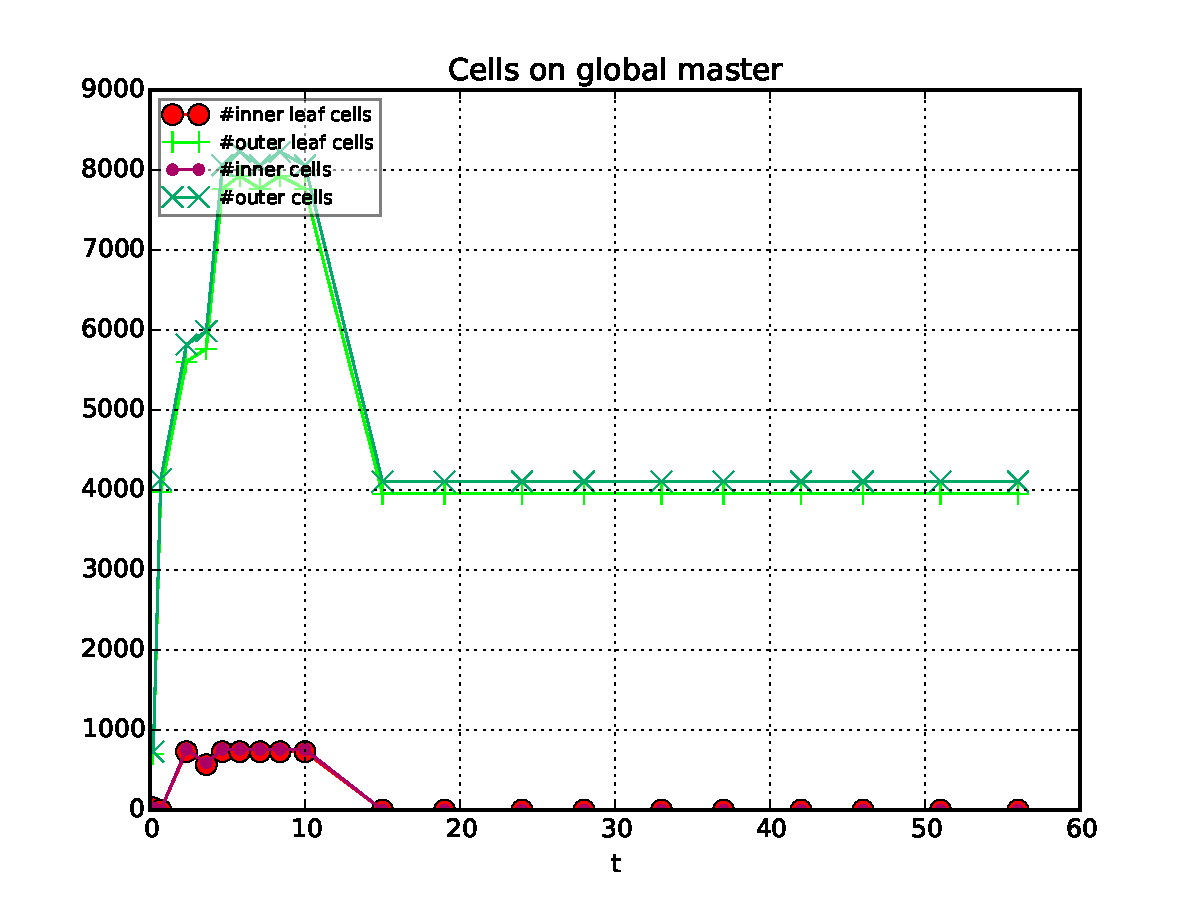
\includegraphics[width=0.5\textwidth]{41_mpi-setup/performance-analysis-output.pdf}
\end{center}



If you identify ranks whose local load decreases incrementally, these are ranks
that step by step fork more of their work to other ranks. 
In principle, this is fine and a result of load balancing. 
For reasonably static setups, it however is irritating: 
why is there such a long setup phase where obviously solely data is
redistributed?

The reason can be found in the semantics of \texttt{createVertex} and
\texttt{touchVertexFirstTime}.
Both operations try to refine the grid around the respective vertex immediately. 
Only if circumstances such as a parallel partitioning running through this
vertex---the refinement instruction then first has be distributed to all ranks
holding a copy of this vertex---do not allow Peano to realise the refinement
immediately, the refinement is postponed to the next iteration.
In many parallel codes, all the refinement calls pass through immediately on
rank 0 before it can spawn any rank.
This leads to the situation that the whole grid is in one sweep built up on the
global master and afterwards successively distributed among the ranks.


Such a behaviour is problematic: the global rank might run out of memory, lots
of data is transferred, and the sweeps over the whole grid on rank 0 are
typically pretty expensive. 
A distributed grid setup is advantageous.

\paragraph{The solution}

To facilitate this, it makes sense to switch from an aggressive
refinement into an iterative grid refinement strategy (one refinement level per
step, e.g.) to allow the rank to deploy work throughout the grid construction
and thus build up the grid in parallel and avoid the transfer of whole grid
blocks due to rebalancing.
Simply move your \texttt{refine()} call from the creational or touch first
events into \texttt{touchVertexLastTime()}:
As a consequence, setting up a (rather regular) grid of depth k requires at least k iterations. 


To find out when a grid has been constructed and balanced completely, the
repository provides an operation. Instead of writing something along the lines

\begin{code}
  repository.switchToSetup();
  repository.iterate();
\end{code}

\noindent
you have to write
\begin{code}
  repository.switchToSetupExperiment();
  do {
    repository.iterate();
  } while ( !repository.getState().isGridBalanced() );
\end{code}



\paragraph{Related pitfalls \& ideas}

As always, the devil is in the details:
\begin{itemize}
  \item  For many load balancing algorithms, it does make sense to create an
  initial grid of depth $\hat k <k$ on your rank 0 before you do any load
  balancing. This allows the load balancing metric to get a first idea about
  what the grid will look like and then to trigger an appropriate load
  balancing. To do so, you can require two mappings: one that builds up the grid
  in \texttt{createVertex} and \texttt{touchVertexFirstTime} up to a certain
  finest level, and one additional mapping that incrementally creates the
  additional mappings and thus allows for a fine-tuned load balancing.
  \item Once all ranks have obtained `their' partition, it does not make sense
  to continue to build up at most one grid level per sweep. In this case, you
  have to reliase an inverse pattern compared to the pattern sketched in the
  first bullet point. Such a situation is easy to spot: it typically
  materialises in a slow increase of total/global vertices while the fork
  statistics show that no forks happen anymore. Compare the two plots below:
  \begin{center}
    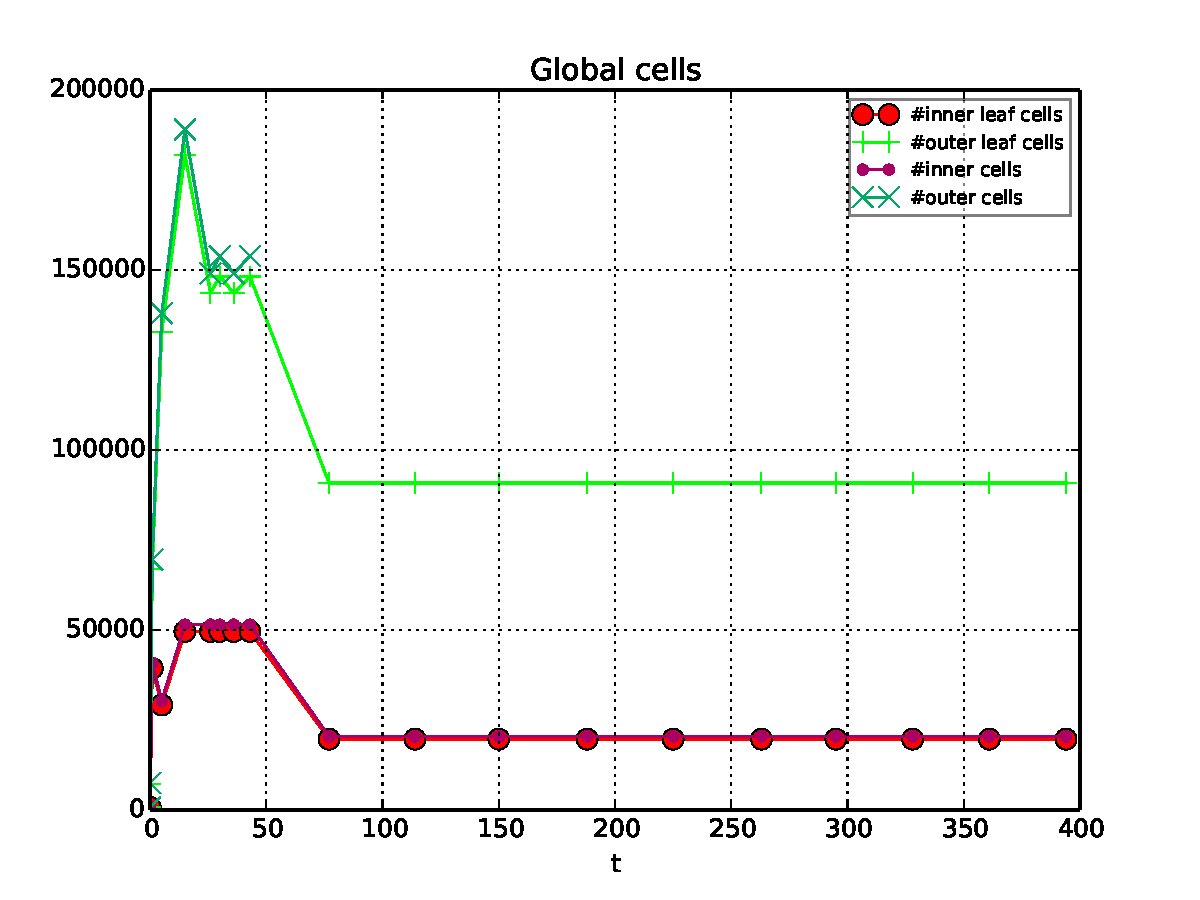
\includegraphics[width=0.4\textwidth]{41_mpi-setup/grid-construction.pdf}
    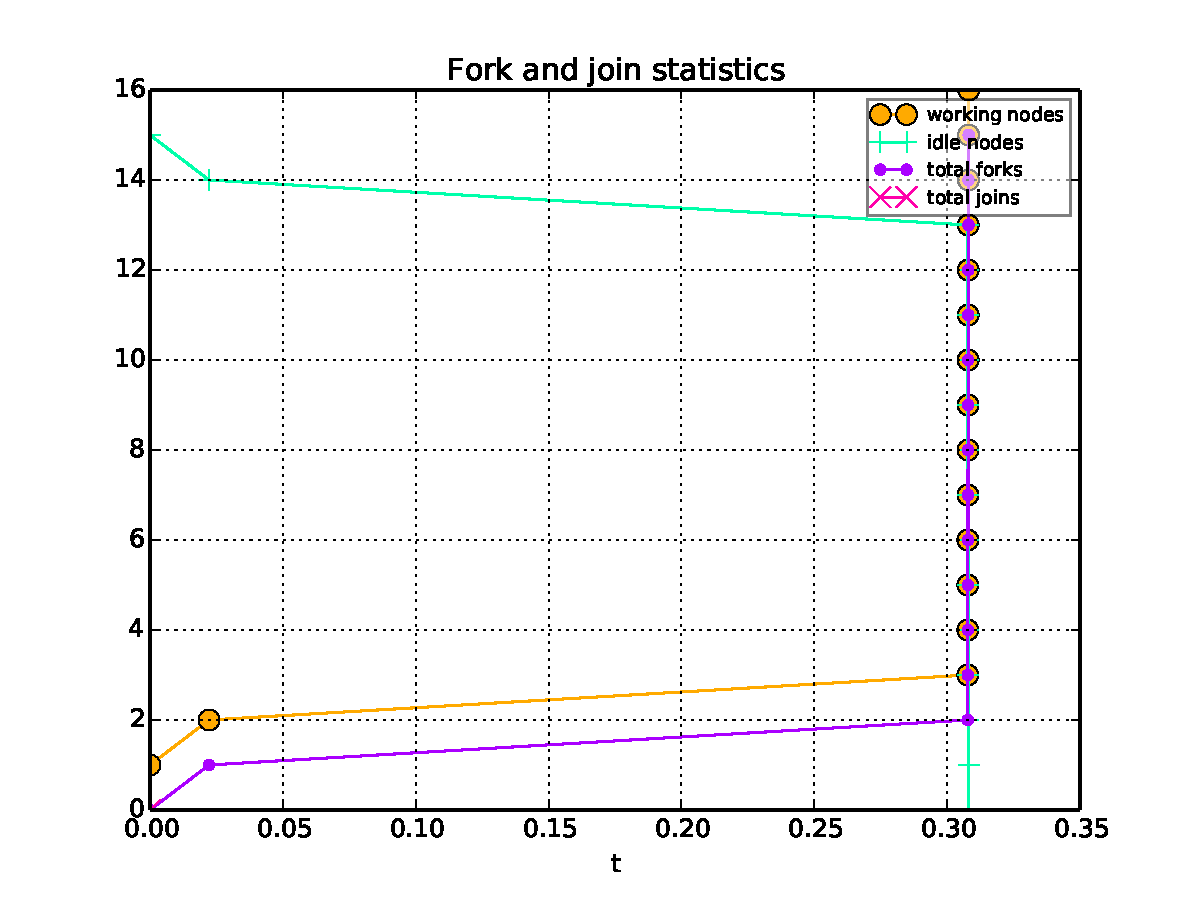
\includegraphics[width=0.4\textwidth]{41_mpi-setup/fork-behaviour.pdf}
    \\
    {
    \footnotesize
    The grid construction requires about 80s while the last forks are tracked
    at t=0.3s. From hereon, one could build up the grid one sweep.
    }
  \end{center}
  \begin{remark}
    Peano parallel code offers an operation \texttt{enforceRefine()} on
    the vertices that you can use to tackle this problem. Use with care and 
    read through the documentation in code.
  \end{remark}
  \item Everytime you rebalance your grid, Peano disables dynamic load balancing
  for a couple of iterations (three or four). Throughout these iterations, it
  can recover all adjacency information if the grid itself changes as well.
  Consequently, it does make sense to add a couple of adapter runs after each
  grid modification that to not change the grid structure: When you know that
  you have an adapter that changes the grid, apply afterwards an adapter that
  does not change the grid for a couple of times. This way, you ensure that no
  mpi rank runs out of memory. The grid generation does not overtake the rebalancing.
  \item If you are using the heap data structure, it furthermore makes sense to split up
the initialisation into a grid setup and a data struture initialisation.
You balance and distribute the grid setup following the recommendations above
and then in one additional sweep initialise the heap.
You initialise the heap as late as possible and thus avoid unneccesary
administrative overhead.
\end{itemize}

  \section{MPI quick tuning}


\chapterDescription
  {
    Around 15 minutes.
  }
  {
    A working MPI code.
  }


This section collects a couple of really primitive measurements to make your
code faster.

\subsection{Filter out log statements}

It is probably to simple to mention, but all our teams from time to time forget
this. 
One of the major things slowing down codes is writing to the terminal. 
So adding a few additional log filters can significantly speed up your code.



\subsection{Switch off load balancing}

Most of Peano's load balancing algorithms (at least the ones coming along with
the standard package) rely on a central node pool.
If a rank decides that it would be advantageous to split up its domain, it sends
a request to the first rank whether there are any idle nodes available.
If your code already uses all ranks, this is a time consuming process that
suffers from latency.
If you know a prior that the load balancing is static and no further splits of
subdomains are possible, it does make sense to switch the load balancing off.
There is a routine \texttt{activateLoadBalancing} operation on the load
balancing oracle to do so.

This operation has to be called on each individual rank, i.e.~you can switch 
the load balancing on and off on a rank-per-rank basis. There are basically two
variants/patterns to disable the load balancing:
\begin{enumerate}
  \item You may introduce a new mapping that does nothing besides switching the
  load balancing off (typically in \texttt{beginIteration}). You then merge this
  mapping into your other adapters.
  \item You add a new bool to your state. In the global runner you set this
  boolean flag once you want to switch the load balancing off. The state then is
  successively propagated to the workers. In \texttt{beginIteration}, you
  analyse this bool (in any mapping) and you switch off the load balancing if
  the flag is set.
\end{enumerate}

Peano also offers the opportunity to invoke a
global step on all ranks prior to an \texttt{iterate} call.
This feature can be used to switch off the load balancing, too:

\begin{code}
void picard::runners::Runner::runGlobalStep() {
  peano::parallel::loadbalancing::Oracle::getInstance().activateLoadBalancing(false);
}


int picard::runners::Runner::runAsMaster(...) {
  ...
  
  repository.runGlobalStep(); // on all other ranks
  runGlobalStep();            // and locally, too
}
\end{code}

\noindent
As clarified in the documentation of the operations (see the autogenerated
header files of your repository, e.g.), you have to be careful if you follow
this variant:
You are never allowed to run a global step if any rank is involved in a join or
fork. 


  
% Die ganzen Optimisation Flags; eher tuning?

%  \section{Multicore support} 
%  \section{MPI with spacetree-associated data} 
%  \section{MPI with data on the heap} 
%  \section{Multicore load balancing} 
%  \section{MPI load balancing} 
%  \section{Tuning the single core performance} 
 

\end{document}
